\chapter{Recurring functional sub-networks during ictal and interictal periods}
\label{ch:mapsubnet}

% the code below specifies where the figures are stored
\ifpdf
    \graphicspath{{chapters/ch4_figures/PNG/}{chapters/ch4_figures/PDF/}{chapters/ch4_figures/}}
\else
    \graphicspath{{chapters/ch4_figures/EPS/}{chapters/ch4_figures/}}
\fi


% ----------------------------------------------------------------------
%: ----------------------- content ----------------------- 
% ----------------------------------------------------------------------
\section{Abstract}
Patients with drug-resistant, neocortical epilepsy suffer from spontaneous seizures, which originate in cortical structures that could also sub-serve normal function. Current clinical practice for localizing seizure-generating brain regions entails monitoring changes from background, interictal patterns of neural activity as seizure begin. A significant challenge with this approach is discerning which cortical pathways lead to seizures and which are important for normal function. We developed a novel technique to disentangle functional sub-networks comprising cohesive cortical pathways from time-varying functional networks constructed from intracranial recordings. Using a consensus clustering scheme, we identified stable clusters of functional pathways expressed during ictal and interictal periods. Our results suggest that cortical pathways involving seizure-onset areas are expressed during both periods and may be predicted by the average strength of connections in the sub-network. Meanwhile, the time-varying expression of cortical pathways from functional sub-networks differentially explains network dynamics during ictal and interictal periods. We found that functional sub-networks are more transiently expressed during ictal periods and more persistently expressed during interictal periods. Collectively, our observations implicate a complex and consistent functional relationship between seizure-generating and ``normal'' structures. Although dysfunction within the epileptic network persists during interictal periods, pathologic regions of the network can be reliably predicted many hours before seizures begin.

\section{Introduction}
For approximately 60 million epilepsy patients, recurring, spontaneous seizures have crippling impact on daily life. In $\approx26\%$ of patients, drivers of seizure activity have been linked to abnormal focal networks located in the neocortex or mesial temporal structures \cite{siegel2001medically}. While the most common treatment strategy is surgical resection to remove cortical tissue generating seizures, newer options such as laser ablation and implantable devices have emerged to selectively target abnormal regions in epileptic networks \cite{fisher2010electrical, morrell2011responsive, tovar-spinoza2013use, medvid2015current}. When discrete lesions coinciding with abnormal electrophysiology are not evident on MRI, only $\approx40\%$ of patients attain seizure freedom following resective surgery. To improve post-surgical outcome, clinicians are increasingly interested in tailoring novel, targeted therapy to affect network regions involved in seizure generation and spread \cite{kutsy1999ictal}. 

To describe mechanisms of seizure generation and evolution, several prior studies have studied the dynamics of epileptic networks, where network nodes are intracranial sensors measuring the electrocorticogram (ECoG) and network connections are statistical relationships between sensors \cite{friston2011functional, hutchison2013dynamic}. Most recent approaches map topologically important network regions within clinically-defined seizure-onset zones and track network dynamics during ictal (seizure) and interictal (normal baseline) epochs \cite{wendling2003epileptic, jerger2005multivariate, schindler2006assessing, schindler2008evolving, kramer2010coalescence, jiruska2012synchronization, burns2014network}. Network hubs of strong connectivity have also emerged adjacent to seizure-onset zones and may localize broader epileptogenic regions \cite{schevon2007cortical, zaveri2009localization-related, rummel2013systems-level, weiss2013ictal, geier2015how}. Together, these studies reveal that network dysfunction underlies complex interactions between drivers of pathologic seizure activity and functional pathways linking cortical regions and that evidence of abnormality exists well before clinically-manifested seizures. This theory aligns well with the popular perspective that the brain is comprised of a number of modular functional sub-networks, recruiting different cortical regions, of which a subset are likely to be expressed at any given time based on functional demand \cite{deco2011dynamical, deco2011emerging, hansen2015functional}. Which begs the following questions: (i) Are functional sub-networks expressed during phases of ictal epochs similar to those expressed during baseline, interictal epochs, and (ii) Do functional sub-networks have a stereotypic pattern of temporal expression that differentiates their mechanism of cortical recruitment between ictal and interictal epochs?
 
In this work, we applied a novel approach for disentangling functional sub-networks and their temporal likelihood of expression to answer the general question: "How are functional pathways differentially expressed during ictal and interictal epochs?" We hypothesize that a common set of cortical pathways underlie functional communication during ictal and interictal epochs, but that the temporal expression of these pathways is different between the two epochs. We posit that stereotypic network architecture might explain why interictal epileptiform activity follows propagation pathways reminiscent to seizure onset and evolution \cite{alarcon1997origin, lai2007cortical, schevon2009spatial, wu2010removing, wilke2009identification,korzeniewska2014ictal}. Therefore, functional sub-networks that connect different cortical regions during normal function may coincide with pathways responsible for seizure initiation and spread. Our results support this hypothesis, demonstrating that functional sub-networks during interictal epochs predict the stereotypic sub-networks expressed during different stages of ictal epochs. Although similar functional pathways phenotype ictal and interictal network architecture, the time-varying expression of sub-networks differentiate the two epochs.

\section{Results}
To disentangle functional sub-networks and their time-varying expression from epileptic brain, we retrieved ECoG recorded during ictal and interictal epochs from 22 neocortical epilepsy patients undergoing routine pre-surgical evaluation of their epilepsy (see \textbf{Table~{\ref{ch4:tab1}}} for patient-specific information) through the \textit{International Epilepsy Electrophysiology Portal} (IEEG Portal, http://www.ieeg.org). We defined an ictal epoch as the period of ECoG signal between -- seizure-onset -- as characterized by the earliest electrographic change (EEC) \cite{litt2001epileptic} -- and seizure termination and an interictal epoch as a continuous 5 minute period of ECoG signal at least 2 hours preceding or following seizure-onset. We analyzed all possible interictal epochs, which amounted to $105\pm17$ hours of ECoG signal per patient.

In each epoch, we estimated weighted functional connectivity using a normalized cross-correlation metric (see \textit{Methods}) applied to non-overlapping, 1s time windows of ECoG (\textbf{Fig.~\ref{ch4:fig1}}). This procedure results in a symmetric, $N \times N$ \textit{connectivity matrix} (specifying $\mfrac{N(N-1)}{2}$ unique connections in the upper or lower triangle of the symmetric connectivity matrix), where $N$ is the number of network nodes, for each of $T$ time windows analyzed. The pattern of unique network connections over all time windows in the epoch is a \textit{configuration matrix} of size $\mfrac{N(N-1)}{2} \times T$.

To extract functional sub-networks from the epileptic network model, we applied a sub-network learning technique called \textit{non-negative matrix factorization (NMF)} to the configuration matrix (see \textit{Methods}). This technique enabled us to soft-partition the time-varying network configuration into modular sub-networks with time-varying expression coefficients. Each sub-network is an additive component of the original network, representing communication pathways between a subset of network regions, that is accompanied by time-varying expression coefficients, measuring the degree to which each sub-network is expressed at a given point in time.

To better understand normal and dysfunctional architecture in the epileptic network, we study the functional sub-networks and time-varying expression coefficients during ictal and interictal epochs.

\begin{table}[H]
    \scriptsize
    \centering
    \begin{tabular}{|x{2cm}|x{0.5cm}|x{0.75cm}|x{2cm}|x{1.5cm}|x{1.25cm}|x{1cm}|x{1cm}|x{1.40cm}|}
        \hline
        Patient\newline (IEEG Portal) & Sex & Age & Seizure Onset & Etiology & Seizure Type & Seizures (N) & Imaging & Outcome \\ \hline \hline
        \verb|HUP64_phaseII| & M & 03/20 & Left frontal & Dysplasia & CP+GTC & 01 & L & ENGEL-I\\ \hline
        \verb|HUP65_phaseII| & M & 02/36 & Right temporal & Auditory reflex & CP+GTC & 03 & N/A & ENGEL-I\\ \hline
        \verb|HUP68_phaseII| & F & 15/26 & Right temporal & Meningitis & CP, CP+GTC & 05 & NL & ENGEL-I\\ \hline
        \verb|HUP70_phaseII| & M & 10/32 & Left perirolandic & Cryptogenic & SP & 08 & L & NR\\ \hline
        \verb|HUP72_phaseII| & F & 11/27 & Bilateral left & Mesial temporal sclerosis & CP+GTC & 01 & L & NR\\ \hline
        \verb|HUP73_phaseII| & M & 11/39 & Anterior right frontal & Meningitis & CP+GTC & 05 & NL & ENGEL-I\\ \hline
        \verb|HUP78_phaseII| & M & 00/54 & Anterior left temporal & Traumatic injury & CP & 05 & L & ENGEL-III\\ \hline
        \verb|HUP79_phaseII| & F & 11/39 & Occipital & Meningitis & CP & 01 & L & NR\\ \hline
        \verb|HUP86_phaseII| & F & 18/25 & Left temporal & Cryptogenic & CP+GTC & 02 & NL & ENGEL-II\\ \hline
        \verb|HUP87_phaseII| & M & 21/24 & Frontal & Meningitis & CP & 02 & L & ENGEL-I\\ \hline
        \verb|Study 004-2|   & F & 14/27 & Right temporal occipital & Unknown & CP+GTC & 01 & NL & ILAE-IV\\ \hline
        \verb|Study 006|     & M & 22/25 & Left frontal & Unknown & CP & 02 & NL & NR\\ \hline
        \verb|Study 010|     & F & 00/13 & Left frontal & Unknown & CP & 02 & L & NF\\ \hline
        \verb|Study 011|     & F & 10/34 & Right frontal & Unknown & CP, CP+GTC & 02 & NL & NF\\ \hline
        \verb|Study 016|     & F & 05/36 & Right temporal orbitofrontal & Unknown & CP+GTC & 03 & NL & ILAE-IV\\ \hline
        \verb|Study 019|     & F & 31/33 & Left temporal & Unknown & CP+GTC & 15 & NL & ILAE-V\\ \hline
        \verb|Study 020|     & M & 05/10 & Right frontal & Unknown & CP+GTC & 04 & NL & ILAE-IV\\ \hline
        \verb|Study 023|     & M & 01/16 & Left occipital & Unknown & CP & 04 & L & ILAE-I\\ \hline
        \verb|Study 026|     & M & 09/09 & Left frontal & Unknown & CP & 10 & NL & ILAE-I\\ \hline
        \verb|Study 031|     & M & 05/05 & Right frontal & Unknown & CP+GTC & 05 & NL & NF\\ \hline
        \verb|Study 033|     & M & 00/03 & Left frontal & Unknown & GA & 07 & L & ILAE-V\\ \hline
        \verb|Study 037|     & F & 45/?? & Indeterminate & Unknown & CP & 02 & NL & NR\\ \hline
    \end{tabular}
    \caption[Patient data set for Chapter \ref{ch:mapsubnet}]{\textbf{Patient information.} Patient data sets accessed through IEEG Portal (http://www.ieeg.org). Age (years) at first reported onset and at phase II monitoring. Localization of seizure onset and etiology is clinically-determined through medical history, imaging, and long-term invasive monitoring. Seizure types are SP (simple-partial), CP (complex-partial), CP+GTC (complex-partial with secondary generalization), or GA (generalized atonic). Counted seizures were recorded in the epilepsy monitoring unit. Clinical imaging analysis concludes L, Lesion; NL, non-lesion. Surgical outcome was based on either Engel score or ILAE score (scale: I-IV/V, seizure freedom to no improvement; NR, no-resection; NF, no follow-up). M, male; F, female. \label{ch4:tab1}}
\end{table}

\begin{figure}[H]
    \centering
    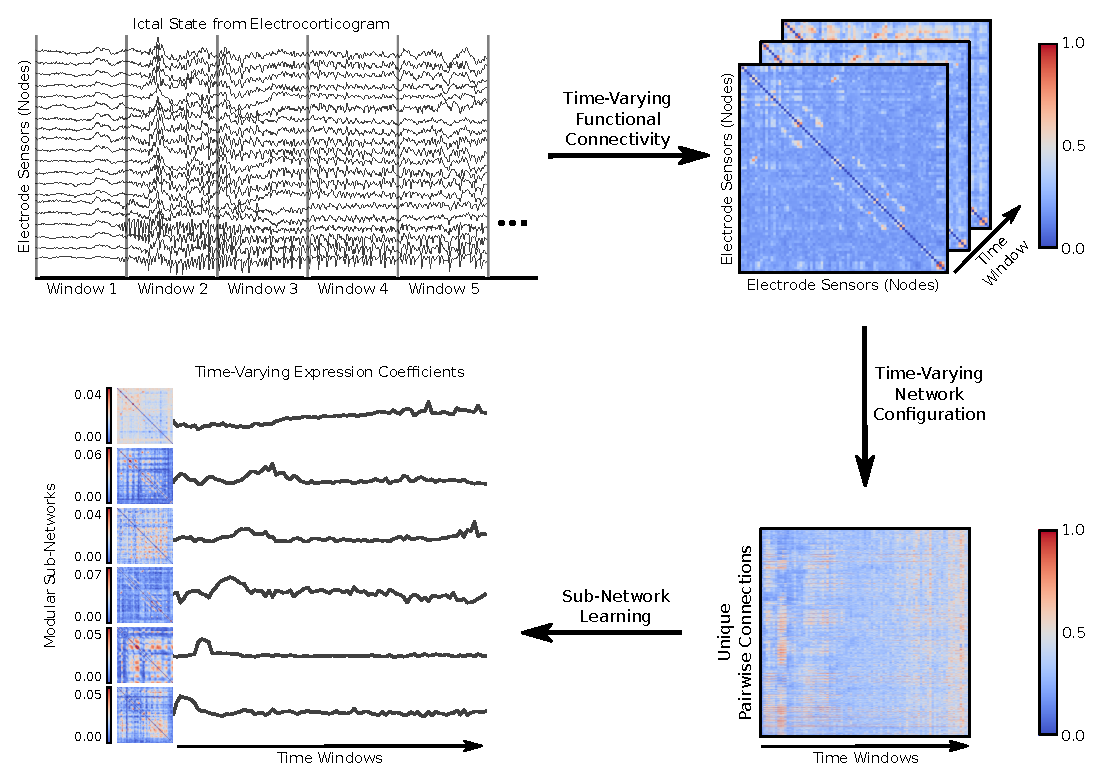
\includegraphics[width=\textwidth]{panel1.eps}
    \caption[Pipeline for disentangling time-varying functional sub-networks]{\textbf{Sub-network learning pipeline for dynamic epileptic networks.} (\textit{Top Left}) We identify ictal and interictal epochs from ECoG signals collected from patients with drug-resistant neocortical epilepsy implanted with intracranial electrodes. An ictal epoch is the period between seizure-onset -- as characterized by the earliest electrographic change (EEC) \cite{litt2001epileptic} -- and seizure termination. An interictal epoch is a continuous, 5 minute period at least 2 hours preceding or following seizure-onset. To measure time-varying functional networks, we divide each epoch into 1s time windows and estimate connectivity in each time window. In our model, each electrode sensor is a network node, and weighted functional connectivity between sensors, interpreted as degree of synchrony, is represented as a network connection. (\textit{Top Right}) For each epoch, we estimated functional connectivity by applying a magnitude normalized cross-correlation between each pair of sensor time series in each time window). (\textit{Bottom Right}) For time-varying functional connectivity, we extract all unique connections between nodes and concatenate over time windows to generate a time-varying network configuration matrix. (\textit{Bottom Left}) We apply \textit{NMF} to the time-varying configuration matrix from each epoch, resulting in a set of co-expressed network regions, sub-networks, with associated expression coefficients for each time window. \label{ch4:fig1}}
\end{figure}

\subsection{Ictal Network Architecture Emerges During Interictal epochs}
Are modular sub-networks expressed during ictal epochs quantifiably similar to those expressed during interictal epochs? To answer this question, we developed a consensus clustering technique to evaluate the degree of similarity between sub-networks of ictal and interictal epochs (see \textit{Methods}). We first generated an ensemble of sub-networks, learned from time-varying functional connectivity of each patient's ictal and interictal epochs. This procedure yielded a patient-specific \textit{ensemble matrix} representing the unique pairwise connectivity between network nodes for every sub-network learned over all epochs (\textbf{Fig.~\ref{ch4:fig2}}). To compute a null distribution of sub-networks for each epoch, we applied a randomly weighted, linear combination of the sub-networks and constructed a \textit{surrogate ensemble matrix}.

Using the true and surrogate ensemble matrices, we next asked whether sub-networks of ictal and interictal epochs reliably cluster together. To test for co-clustering probability between ictal and interictal epochs in each patient, we applied a second stage NMF to the ensemble matrix and tracked the number of times each possible pair of sub-networks were assigned in the same cluster over 100 random initializations. We optimized the number of sub-network clusters per patient by repeating the co-clustering procedure over a range of number of clusters (see \textit{Supplemental Information}). For each patient, this technique yielded a co-clustering probability matrix (\textbf{Fig.~\ref{ch4:fig2}}) capturing the frequency with which pairs of sub-networks over all epochs clustered together. Across the 22 patient cohort, we identified 5 -- 20 clusters consisting of ictal and interictal sub-networks (see \textit{Supplemental Information}). 

\begin{figure}[H]
    \centering
    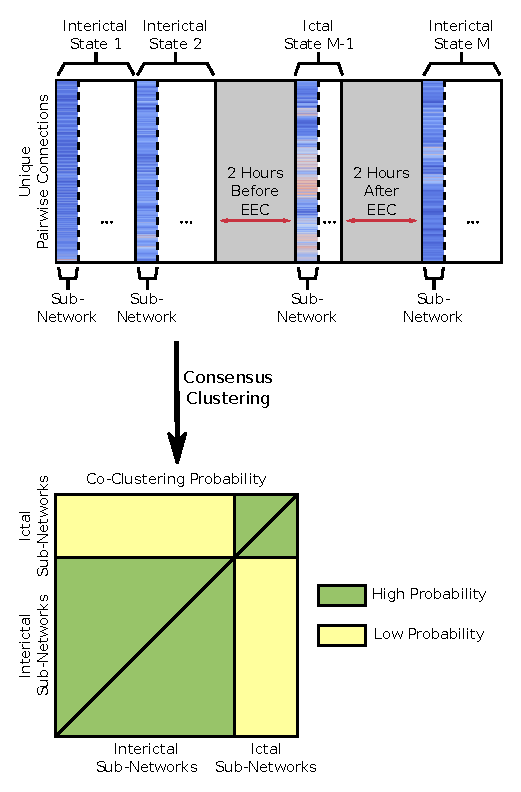
\includegraphics[width=0.5\textwidth]{panel2.eps}
    \caption[Consensus clustering of sub-network ensembles]{\textbf{Consensus clustering for ensemble of sub-networks.} (\textit{Top}) For each patient, we constructed an \textit{ensemble matrix}, representing the $\mfrac{N(N-1)}{2}$ unique connections for each sub-network learned over all ictal and interictal epochs. The ensemble matrix aggregates cortical sub-regions that are expressed during the patients' long-term intracranial recording. We also constructed a \textit{surrogate ensemble matrix} by computing randomly-weighted superposition of sub-networks from each epoch. (\textit{Bottom}) To quantify similarity between cortical sub-regions expressed during interictal and ictal epochs, we employed consensus clustering by applying NMF to the ensemble matrix over a range of number of sub-network clusters each with 100 random initializations. This resulted in a co-clustering probability matrix representing the frequency with which sub-networks from ictal and interictal epochs in the ensemble matrix are clustered together. \label{ch4:fig2}}  
\end{figure}

To analyze the similarity between ictal and interictal sub-networks, we applied multidimensional scaling to project each patient's co-clustering probability matrix on a two-dimensional Euclidean space for true (\textbf{Fig.~\ref{ch4:fig3}A}) and surrogate sub-networks (\textbf{Fig.~\ref{ch4:fig3}B}). This technique projects topographically similar sub-networks closer together (i.e. shorter Euclidean distance). To test whether clusters are significantly more cohesive amongst true sub-networks than surrogate sub-networks, we measured the average Euclidean distance from each sub-network to its cluster centroid, normalized by the distance of the sub-network the population centroid (\textbf{Fig.~\ref{ch4:fig3}C}). Using a One-Way Repeated Measures ANOVA, we found that true clusters are significantly more cohesive than surrogate clusters ($F_{1,21}=1387$, $p<2\times10^{-16}$). This suggests that sub-networks of true clusters are significantly more similar than sub-networks of surrogate clusters. 

Based on our finding of cohesive clustering amongst true ictal and interictal sub-networks, we asked how tightly integrated are ictal sub-networks within their assigned clusters. To quantify cluster integration of ictal sub-networks, as before, we measured the average normalized Euclidean distance from each ictal and interictal sub-network to its cluster centroid, solely for clusters that contained sub-networks of both epochs (\textbf{Fig.~\ref{ch4:fig3}D}). Using a One-Way Repeated Measures ANOVA, we found that ictal sub-networks are significantly more distant from their cluster centroid than interictal sub-networks ($F_{1,21}=11.42$, $p<0.005$). This suggests that ictal sub-networks are less integrated within the cluster than interictal sub-networks. Based on our observation of bridge-like transitions in the two-dimensional projection space of clusters (\textbf{Fig.~\ref{ch4:fig3}A}), we believe ictal sub-networks may represent cortical pathways that lay at the transition between interictal epochs. 

\begin{figure}[H]
    \centering
    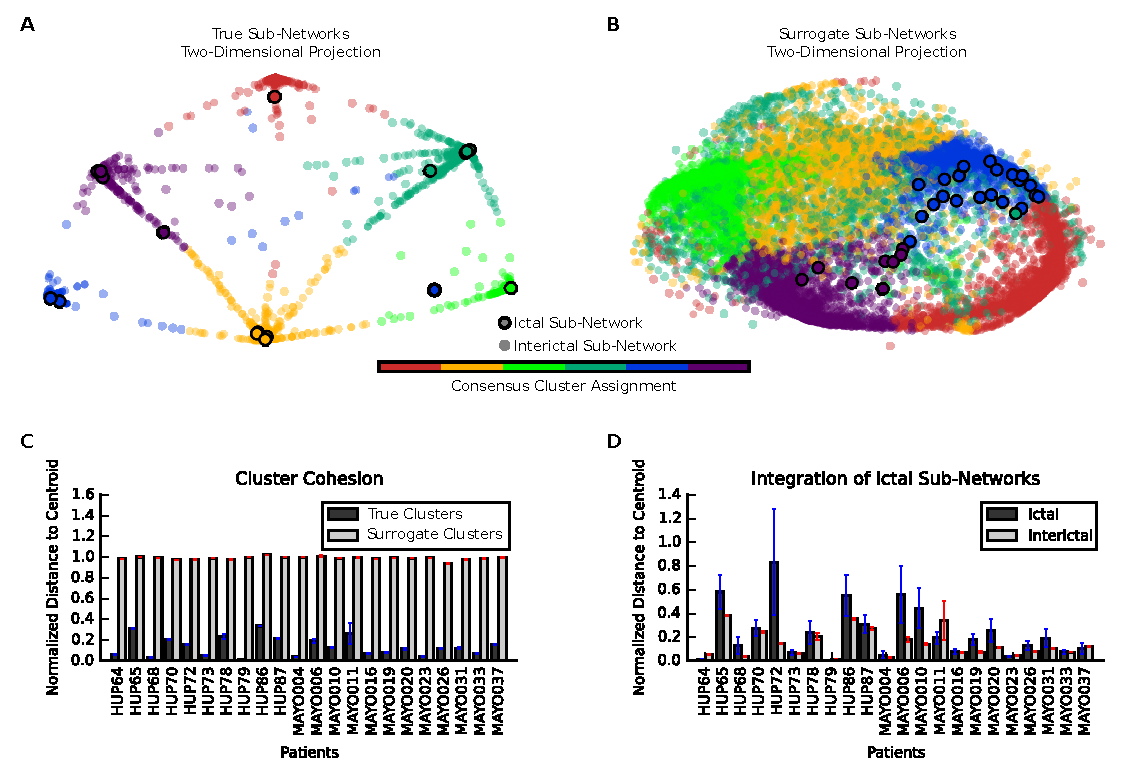
\includegraphics[width=\textwidth]{panel3.eps}
    \caption[Ictal sub-networks recapitulated during interictal epochs]{\textbf{Ictal sub-networks are recapitulated during interictal epochs.} (\textbf{A}) Example two-dimensional projection of one patient's co-clustering probability matrix, where shorter Euclidean distances between circles indicates greater co-clustering probability between expressed sub-networks. Bolded circles represent sub-networks expressed during ictal epochs, and colors represent consensus cluster assignments for each sub-network. (\textbf{B}) Example two-dimensional projection of same patient's surrogate co-clustering probability matrix. The surrogate co-clustering probability matrix, was generated after applying consensus clustering to the surrogate ensemble matrix. (\textbf{C}) Average projection distance from each sub-network to its cluster centroid, normalized by distance to the population centroid, for true and surrogate clusters of each patient. True clusters were significantly more cohesive than surrogate clusters for all 22 patients (One-Way Repeated Measures ANOVA; $F_{1,21}=1387$, $p<2\times10^{-16}$).  (\textbf{D}) Average projection distance from ictal and interictal sub-networks to its cluster centroid, normalized by distance to the population centroid. Ictal sub-networks were significantly further from the cluster centroid than interictal sub-networks (One-Way Repeated Measures ANOVA; $F_{1,21}=11.42$, $p<0.005$) \label{ch4:fig3}}
\end{figure}

\subsection{Interictal Sub-Networks Stereotype Epileptic Network}
In the preceding analyses, we observed that: (i) sub-networks within the same cluster are more similar than sub-networks assigned to other clusters, (ii) ictal sub-networks co-cluster with interictal sub-networks, yet ictal sub-networks tend to be further from the cluster centroid. Next, we investigated to what extent interictal sub-networks can stereotype epileptic network architecture. To address this question, we tested whether interictal sub-networks are capable of predicting pathways related to seizure foci. In accord with routine clinical work-up of patients' epilepsy, a team of neurologists successfully identified the sensors on the seizure-onset zone (SOZ) based on visual inspection of the intracranial recordings. 

We first quantified the extent to which interictal sub-networks express seizure-onset pathways, by computing the \textit{SOZ expression index} as $\mfrac{\bar{C}_\textrm{SOZ}-\bar{C}_\textrm{OUT}}{\bar{C}_\textrm{SOZ}-\bar{C}_\textrm{OUT}}$ -- $\bar{C}_\textrm{SOZ}$ is average connection strength between SOZ nodes in the sub-network and$ \bar{C}_\textrm{OUT}$ is average connection strength between nodes outside the SOZ in the sub-network -- where values range from 0 to 1, representing minimal to strong differential expression between SOZ-SOZ and OUT-OUT connections. To study whether clusters containing interictal sub-networks capture epileptic network architecture, we computed the average SOZ expression index within clusters and sorted the clusters in decreasing order. In an example patient we observed focal expression of SOZ connections in interictal sub-networks with broader expression in ictal sub-networks from the same cluster (\textbf{Fig.~\ref{ch4:fig4}A}). To test whether clusters stereotype interictal sub-networks that express SOZ connectivity, we constructed a linear mixed effects model with no fixed effects and with random effects modeled as intercepts for nested clusters within subjects (\textbf{Fig.~\ref{ch4:fig4}B}). We applied the linear mixed effects model to predict SOZ expression index in true sub-networks and in null sub-networks, where connection strengths within each sub-network were randomly permuted. Using the likelihood ratio test, we found that the observed clusters are more likely to generate true SOZ expression indices ($r^2=0.287$) than null SOZ expression indices ($\tilde{\chi}^2(1)=36091$, $p<2\times10^{-16}$). These results imply that clusters comprised of interictal sub-networks capture network regions involved in seizure-onset, and that some clusters have greater predictive power than others.

While interictal sub-networks can distinguish epileptic network architecture, thus far we only tested the case where we had priori knowledge regarding seizure onset regions. We next asked whether global topological measures can distinctly predict which interictal sub-networks express SOZ connectivity strongly with no prior knowledge of seizure onset regions. To test this hypothesis, we computed and appended the averaged connection strength of each interictal sub-network as a fixed effect to our previous linear mixed effects model (with random effects modeled as intercepts for nested clusters with subjects). Using the likelihood ratio test, we found that the modified linear mixed effects model is significantly more likely to generate the observed values of SOZ expression index than the previous model without fixed effects  ($\tilde{\chi}^2(4)=5952$, $p<2\times10^{-16}$). For our modified model, we evaluated the marginal goodness-of-fit, where average connection strength (fixed effects) alone explain 30.9\%, and the conditional goodness-of-fit, where the full model (fixed effects and random effects) explain 79.6\%, of the overall variance in SOZ expression index amongst interictal sub-networks (\textbf{Fig.~\ref{ch4:fig4}C}). These results presented strong evidence that interictal sub-networks expressing strong SOZ connectivity can be predicted by a global measure of average connection strength. Furthermore, predictability improved by 48.7\% when accounting for clusters of interictal sub-networks that express similar network pathways.

\begin{figure}[H]
    \centering
    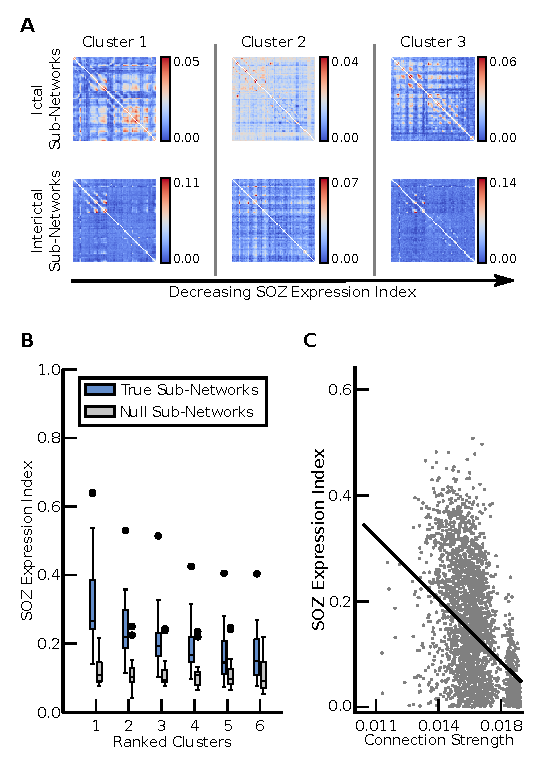
\includegraphics[width=0.5\textwidth]{panel4.eps}
    \caption[Interictal sub-networks predict epileptic network architecture]{\textbf{Interictal sub-networks express emergent architecture of the epileptic network.} (\textbf{A}) First three clusters in order of decreasing SOZ expression index, averaged over all sub-networks within a cluster, for an example patient. Ictal and interictal sub-networks shown are closest to cluster centroids. (\textbf{B}) Distribution of average SOZ expression index over clusters, ranked in decreasing order, from each patient for sub-networks with true (blue) and randomly permuted, null connection strengths (gray). Using a linear mixed effects model to predict SOZ expression index for sub-networks with no fixed effects and with random effects modeled as intercepts for nested clusters within subjects, we found that consensus clusters explain 28.7\% of variance for true SOZ expression index as compared to 17.9\% of variance for null SOZ activation index. (\textbf{C}) Relationship between SOZ expression index and average connection strength in sub-networks from an example patient. Using a linear mixed effects model to predict SOZ expression index with average connection strength as a fixed effect and with random effects modeled as intercepts for nested clusters within subjects, we found that the fixed effects alone explain 29.6\% of the overall variance in SOZ expression index and the full model (fixed effects with random effects) explains 81.4\%. \label{ch4:fig4}}
\end{figure}


\subsection{Functional Sub-Networks Differentially Expressed During Ictal epochs}
We have presented evidence that (i) ictal sub-networks express similar pathways as interictal sub-networks, and (ii) seizure-onset can be predicted by the topology of interictal sub-networks. Logically, we finally ask "If ictal and interictal sub-networks express similar network architecture, how are ictal epochs different from interictal epochs?" 

To answer this question, we analyzed the time-varying expression of sub-networks during ictal and interictal epochs. Based on the understanding that seizures are characterized by a dynamic progression of well-defined epochs, we hypothesized that sub-networks are more transiently expressed, perhaps sequentially, during ictal epochs, and more persistently expressed during interictal epochs. To quantify temporal transience and persistence, we computed the skew of the distribution of time-varying coefficients for each ictal and interictal sub-network, after smoothing with a 5-second moving average filter to reduce spurious noise (\textbf{Fig.~\ref{ch4:fig5}A}). The skew for transient expression was greater than zero, while the skew for persistent expression was less than or equal to zero. Using a One-Way Repeated Measures ANOVA, we found that the skew for ictal time-varying coefficients was significantly greater than for interictal time-varying coefficients ($F_{1,21}=18.81$, $p<0.001$). These results suggest that ictal sub-networks are more transiently expressed than interictal sub-networks, and explains how similar cortical pathways are differentially expressed between ictal and interictal epochs.  

 \begin{figure}[H]
    \centering
    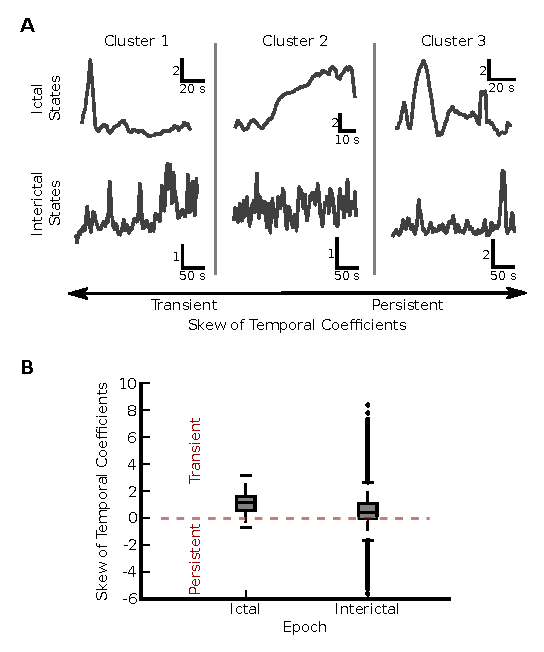
\includegraphics[width=0.5\textwidth]{panel5.eps}
    \caption[Persistent and transient temporal expression of functional sub-networks]{\textbf{Persistent and transient temporal expression differentiates ictal and interictal epochs.} (\textbf{A}) First three clusters in order of increasing skew of temporal coefficients, averaged over all sub-networks within a cluster, for an example patient. Sub-networks with smaller skew in their temporal coefficients are expressed more \textit{persistently} as compared to epochs that are expressed more \textit{transiently}. Temporal coefficients for ictal and interictal sub-networks shown are closest to cluster centroids. (\textbf{B}) Distribution of skew of temporal coefficients for all ictal and interictal sub-networks in an example patient. Using a One-Way Repeated Measures ANOVA, we found that the skew for ictal sub-networks is significantly greater than the skew for interictal sub-networks ($F_{1,21}=18.81$, $p<0.001$). These results suggest that the similar network pathways expressed during ictal and interictal epochs, undergo more transient expression during ictal epochs and are persistent during interictal epochs. \label{ch4:fig5}}
\end{figure}


\section{Discussion}
In this work we asked, "Are similar cortical pathways expressed during ictal and interictal epochs?" To answer this question, we designed and applied a novel tool to disentangle sub-networks and their time-varying expression from dynamic functional connectivity. Our work supports the notion that ictal and interictal epochs traverse a similar set of cortical pathways, but differ in how those pathways are expressed over time. 

\subsection{Modular Cortical Pathways Comprise Epileptic Network Architecture}
A common notion in epilepsy is that isolated cortical regions emit epileptiform activity that can generate seizures. However, network theorists now believe that dysfunction may, in part, arise when epileptiform activity between cortical regions interact, creating the "perfect storm" that leads to seizures. Previous studies have identified discrete network states that describe shifts in the global interactions between all cortical regions \cite{rummel2013systems-level, burns2014network}.  However, these approaches assume that all pathways in the network switch state simultaneously and discretely

Building upon prior work \cite{eavani2013unsupervised, leonardi2013principal, leonardi2014disentangling}, in this study we disentangled the epileptic network into modular sub-networks, or cohesive cortical pathways, that function separately. Logically, different cortical pathways may be variably and continuously expressed to meet functional demand. Our results demonstrated that the epileptic network expresses a small set of functional sub-networks that recur during ictal and interictal epochs. We speculate that the epileptic network consists of stable cortical pathways that contribute to normal function during interictal epochs, and seizure onset and evolution during ictal epochs. Such a theory is corroborated by our finding that these sub-networks are expressed persistently during interictal epochs and transiently during ictal epochs.  


\subsection{Predicting Pathways of the Epileptic Network}
We observed that functional pathways forming the epileptic network are highly predicted by average connection strength and topological clustering of interictal sub-networks. While our results agree with prior studies demonstrating network synchrony is predictive of seizure onset regions during interictal epochs \cite{warren2010synchrony, korzeniewska2014ictal}, we also observed cortical pathways connecting regions outside seizure onset areas that may lead to broader dysfunction \cite{schevon2007cortical, zaveri2009localization-related, weiss2013ictal, rummel2013systems-level}.

Interestingly, these results suggest that functional connectivity linking seizure-onset regions are sustained over long periods of time and persist during functionally normal brain epochs. The appearance of dysfunctional pathways linking cortical regions during interictal epochs can potentially impact cognitive performance in patients with epilepsy. The approach we developed can be used to study looming questions regarding the complex network interactions between epileptic and eloquent cortical regions.

\paragraph{Methodological Limitations and Extensions}
The first important clinical consideration related to this work is the sampling error inherent in any intracranial implantation procedure. Any of the techniques used to map epileptic brain usually yield incomplete representations of the epileptic network. As a consequence, the sub-networks we measured may represent just a portion of larger cortical pathways that extend further throughout the brain.

Secondly, our methods of predicting epileptic network architecture from interictal epochs relies on accurate delineation of seizure-onset regions. Because of sampling error and variability in clinical decision-making, the seizure-onset region may be under or oversampled. However, we believe the high correlation between our model and observed connectivity within seizure-onset regions is reliable based on rigorous statistical testing. Our belief is that unsupervised algorithms to objectively localize network structures may reduce sampling error in the future. 

\subsection{Clinical Impact}
Mapping architecture of the epileptic network presents significant challenges for clinicians. In patients with neocortical epilepsy, we showed that cortical pathways expressed during seizures are highly similar to those pathways traversed during normal function. These findings are relevant for (i) optimizing treatment strategies to reduce dysfunction and preserve normal function and (ii) reducing morbidity and mortality associated with extended duration of invasive intracranial electrode implantation. By predicting seizure-onset regions from interictal epochs, clinical monitoring may be shortened, or potentially even conducted intraoperatively during implant phase. 

\section{Methods}
\subsection{Patient Data Sets}
\subsubsection{Ethics Statement}
All patients included in this study gave written informed consent in accordance with the Institutional Review Board of the University of Pennsylvania.

\subsubsection{Electrophysiology Recordings}
Twenty-two patients undergoing surgical treatment for medically refractory epilepsy believed to be of neocortical origin underwent implantation of subdural electrodes to localize the seizure onset zone after noninvasive monitoring was indeterminate. De-identified patient data was retrieved from the online International Epilepsy Electrophysiology Portal (IEEG Portal) \cite{wagenaar2013multimodal}. ECoG signals were recorded and digitized at either 512 Hz (Hospital of the University of Pennsylvania, Philadelphia, PA) or 500 Hz (Mayo Clinic, Rochester, MN) sampling rate. Surface electrode (Ad Tech Medical Instruments, Racine, WI) configurations, determined by a multidisciplinary team of neurologists and neurosurgeons, consisted of linear and two-dimensional arrays (2.3 mm diameter with 10 mm inter-contact spacing) and sampled the neocortex for epileptic foci (depth electrodes were first verified as being outside the seizure onset zone and subsequently discarded from this analysis). Signals were recorded using a referential montage with the reference electrode, chosen by the clinical team, distant to the site of seizure onset and spanned the duration of a patient's stay in the epilepsy monitoring unit.

\subsubsection{Description of Ictal and Interictal epochs}
Ictal epochs were identified by a team of neurologists as a part of routine clinical work and spanned the period between clinically-marked earliest electrographic change (EEC) \cite{litt2001epileptic} and termination. Interictal epochs spanned 5 minutes in duration and were at least two hours removed from any ictal onset. We analyzed all possible interictal epochs from patient recordings. 

\subsection{Extracting Time-Varying Functional Networks}
Signals from each epoch were divided into $1$-second, non-overlapping, wide-sense stationary time windows in accord with other studies \cite{kramer2010coalescence} and subsequently pre-processed. To test the biasing effect of high-amplitude spiking on signal connectivity measurements, we also investigated windows $0.5$-seconds in duration to sample more of the non-biasing temporal space and found similar results. In each time window, signals were re-referenced to the common average reference \cite{kramer2010coalescence, towle1999electrocorticographic} to account for variation in reference location across patients and to avoid broad field effects that may bias connectivity measurements erroneously in the positive direction. Each window was filtered at 60 Hz to remove line-noise, and low-pass and high-pass filtered at 120 Hz and 1 Hz, respectively, to account for noise and drift. To limit sources of volume conduction from introducing spurious connectivity, we pre-whiten signals in each window using a first-order autoregressive model to account for slow dynamics. This accomplishes two goals: (i) flattening of the signal power spectrum to enhance higher-frequency content that contains local neural population dynamics that is less affected by volume conduction, and (ii) decreases the influence of independent node dynamics when computing correlation-based connectivity measurements \cite{towle1999electrocorticographic, bullmore2001colored, lund2006non-white, arbabshirani2014impact}.

Time-varying functional networks were formed by applying a normalized cross-correlation similarity function $\bs{\rho}$ between the time series of two sensors in the same time window using the formula
    \begin{eqnarray}
        \bs{\rho}_{\mb{xy}}(\mb{k}) = \underset{\tau}{\operatorname{argmax}}\:{\mathrm{E}}[(\mb{x_k}(t) - \mu_{\mb{x_k}})(\mb{y_k}(t+\tau) - \mu_{\mb{y_k}})]
    \end{eqnarray}
    where $\mb{x}$ and $\mb{y}$ are signals from one of $\mb{N}$ sensors or network nodes, $\mb{k}$ is one of $\mb{T}$ non-overlapping, one-second time windows, and $\mb{x_{k}}=\mb{y_{k}}=0$. The $\mb{N}$x$\mb{N}$x$\mb{T}$ similarity matrix is also known as a network adjacency matrix $\mb{A}$. In our weighted network analysis approach, we retain and analyze all possible connection weights between nodes.

\subsection{Learning Functional Sub-Networks}
Sub-networks, or cohesive modules of network pathways, were disentangled from time-varying functional connectivity by clustering the time-varying network configuration matrix through an unsupervised learning algorithm called non-negative matrix factorization (NMF) \cite{lee1999learning}. 

For each ictal or interictal epoch, we constructed the time-varying network configuration matrix $\mb{\hat A}$ by unraveling the upper triangle of $\mb{A}$ resulting in the connection weights of $\mfrac{N(N-1)}{2}$ connections across $\mb{T}$ time windows. Using NMF, we approximated $\mb{\hat A}$ by two low-rank, non-negative matrices, such that:
\begin{eqnarray}
    \mb{\hat A} \approx \mb{W}\mb{H}
\end{eqnarray}
where $\mb{W}$ is the sub-network connectivity matrix (with dimensions $\mfrac{N(N-1)}{2} \times k$), and $\mb{H}$ is the time-varying expression coefficients matrix (with dimensions $k \times T$), and $k$ is the optimized number of sub-networks learned. To compute the NMF, we used the alternating non-negative least squares with block-pivoting method and 200 iterations for fast and efficient factorization of large matrices \cite{kim2011fast} and initialized $\mb{W}$ and $\mb{H}$ using the non-negative double singular value decomposition \cite{boutsidis2008svd}. Given our deterministic initialization for the NMF algorithm, we were guaranteed consistent $\mb{W}$ and $\mb{H}$ on any run -- thus we only performed one run of the NMF algorithm per time-varying network configuration matrix (i.e. one run per ictal or interictal epoch).

For each patient, we determined an optimal number of sub-networks $k$ by the following procedure: (i) randomly sampled 30 epochs from the ictal and interictal pool, (ii) applied NMF for $k$ in the range of 2 to 15 sub-networks independently for each epoch, (iii) computed the Frobenius error between $\mb{\hat A}$ and $\mb{W}\mb{H}$ for each $k$, (iv) retained the value for $k$ that occurs at the elbow of the resulting curve (See \textbf{Fig.~\ref{ch4:figS1}} for distribution of $k$ for each patient), (v) used the average $k$ from 30 epochs as the representative number of sub-networks to learn from all ictal and interictal epochs of the patient. In sum, the sub-network learning procedure yielded $M\times\bar{k}$ total sub-networks per patient, where $M$ is the total number of ictal and interictal epochs. 

\subsection{Consensus Clustering of Sub-Network Ensembles}
Consensus clustering is a general method of testing robustness and stability of clusters over many runs of one or more non-deterministic clustering algorithms \cite{monti2003consensus}. In this work, we studied the nature of clusters amongst the $M\times\bar{k}$ sub-networks per patient. First, we compiled sub-networks from all of a patients' epochs and constructed the ensemble matrix $\mb{E}$ (with dimensions $\mfrac{N(N-1)}{2} \times (M \times \bar{k})$). 

To find consensus clusters in $\mb{E}$, we next applied NMF over 100 runs with matrix factors initialized randomly from a uniform distribution between 0 and 1, such that:
\begin{eqnarray}
    \mb{E} \approx \mb{V}\mb{G}
\end{eqnarray}
where $\mb{G}$ represents the likelihood cluster assignment for each sub-network (with dimensions $j \times (M \times \bar{k})$, where $j$ is the number of patient-wide clusters of sub-networks). After every NMF run, we retrieved the cluster assignment with maximum likelihood for each sub-network and counted the number of times each possible pair of sub-networks was assigned to the same cluster -- and by extension the probability that any two sub-networks co-cluster. These probabilities are tabulated in a symmetric co-clustering probability matrix $\mb{P}$ (with dimensions $(M \times \bar{k}) \times (M \times \bar{k})$). For every patient we repeated this process for a range of $j$ between 5 and 20, and used a proportion of ambiguous clustering (PAC) metric to determine the optimal number of clusters $\bar{j}$ \cite{senbabaoglu2014critical}(see \textbf{Fig.~\ref{ch4:figS2}} for optimal PAC distribution for real and surrogate ensemble matrices). Finally, we assigned each sub-network to its consensus cluster by applying one run of NMF, with $\bar{j}$ clusters, to $\mb{P}$, and retrieving the maximum likely clusters as before (see \textbf{Fig.~\ref{ch4:figS3}}). As suggested by previous work, $\mb{P}$ is a similarity matrix \cite{monti2003consensus} that we used to analyze and visualize sub-network clustering via multi-dimensional scaling methods \cite{borg2005modern}. 

\section{Acknowledgments}
AK and BL acknowledge support from the National Institutes of Health through awards \#R01-NS063039, \#1U24 NS 63930-01A1, the Citizens United for Research in Epilepsy (CURE) through Julie's Hope Award, and the Mirowski Foundation. DSB acknowledges support from the John D. and Catherine T. MacArthur Foundation, the Alfred P. Sloan Foundation, the Army Research Laboratory, the Institute for Translational Medicine and Therapeautics, the National Institute of Mental Health through award number 2-R01-DC-009209-11 (Thompson-Schill), and the National Science Foundation awards CRCNS BCS-1441502 and BCS-1430087 through the ENG, CISE, and SBE directorates. The content is solely the responsibility of the authors and does not necessarily represent the official views of any of the funding agencies.

\begin{figure}[H]
    \centering
    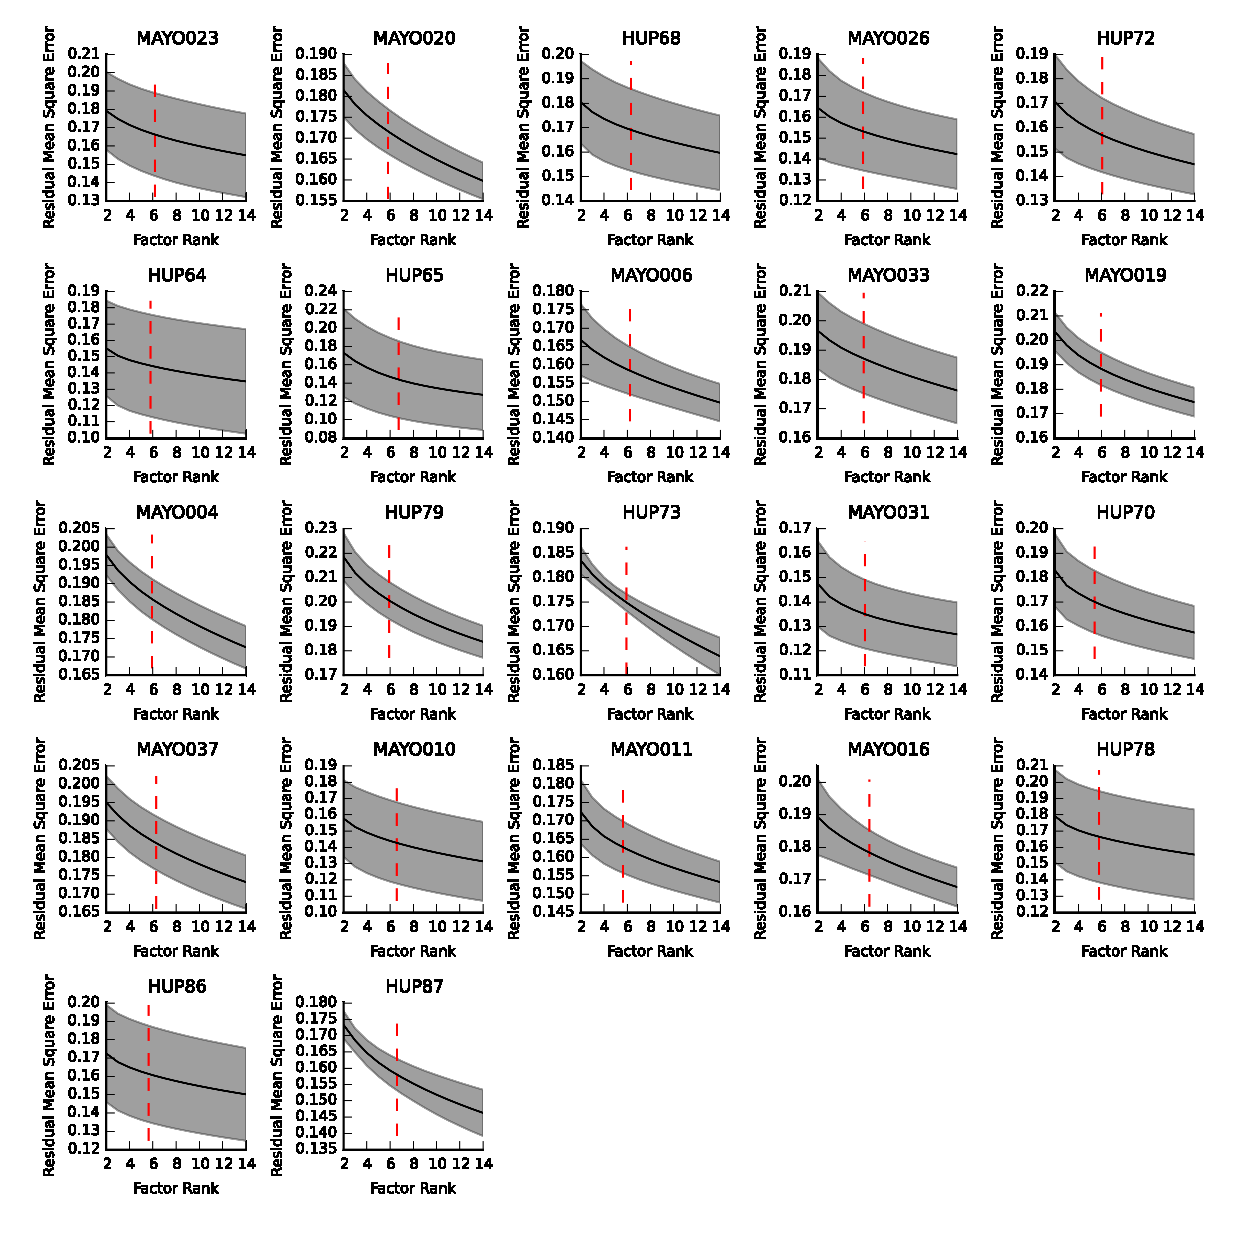
\includegraphics[width=\textwidth]{NMF_factor_optimization.eps}
    \caption[Optimizing number of learned sub-networks]{\textbf{Optimizing number of learned sub-networks.} For each patient, we analyzed the distribution of Frobenius normed error between the network configuration matrix $\mb{\hat A}$ and the learned sub-networks $\mb{W}\mb{H}$ in 30 randomly sampled ictal or interictal epochs. Each graph represents the distribution of error as a function of the number of sub-networks learned $k$. The mean (black) and $\pm1$ standard deviation (gray) over the 30 epochs are plotted. The optimal number of sub-networks $\bar{k}$ for each patient was computed to be the elbow of this curve (dashed red line). \label{ch4:figS1}}    
\end{figure}

\begin{figure}[H]
    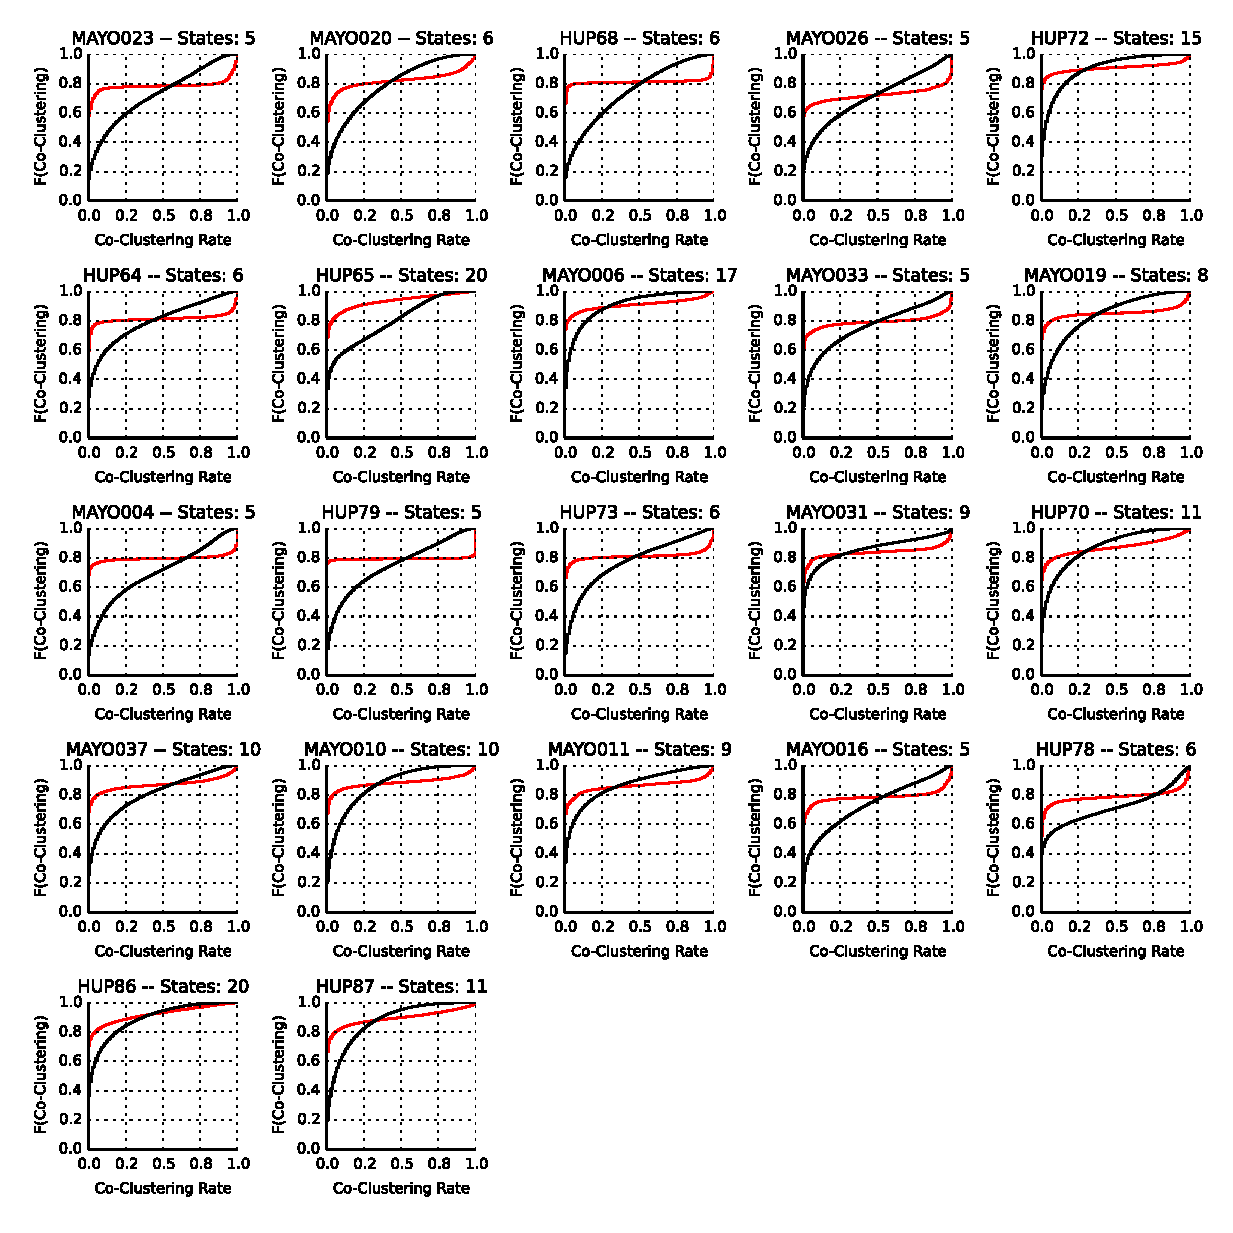
\includegraphics[width=0.9\textwidth]{patient_stateNMF_cdf_pac.eps}
    \caption[Optimizing number of consensus clusters from sub-network ensemble]{\textbf{Optimizing number of consensus clusters from sub-network ensemble.} For each patient, we computed co-clustering probability matrices for a range of number of consensus clusters $j$. To optimize the number of consensus clusters, we computed a cumulative distribution function (CDF) of co-clustering probability for each $j$, quantified the proportion of ambiguous clusters (PAC) as given by $\text{CDF}_j(0.9)-\text{CDF}_j(0.1)$, and retained $\bar{j}$ that resulted in the minimum PAC. The CDF for the optimum number of clusters $\bar{j}$ in red. The CDF for the same number of clusters for the surrogate co-clustering probability matrix is in black. We observed more clustering ambiguity in the surrogate population than the real population. \label{ch4:figS2}}
\end{figure}

\begin{figure}[H]
    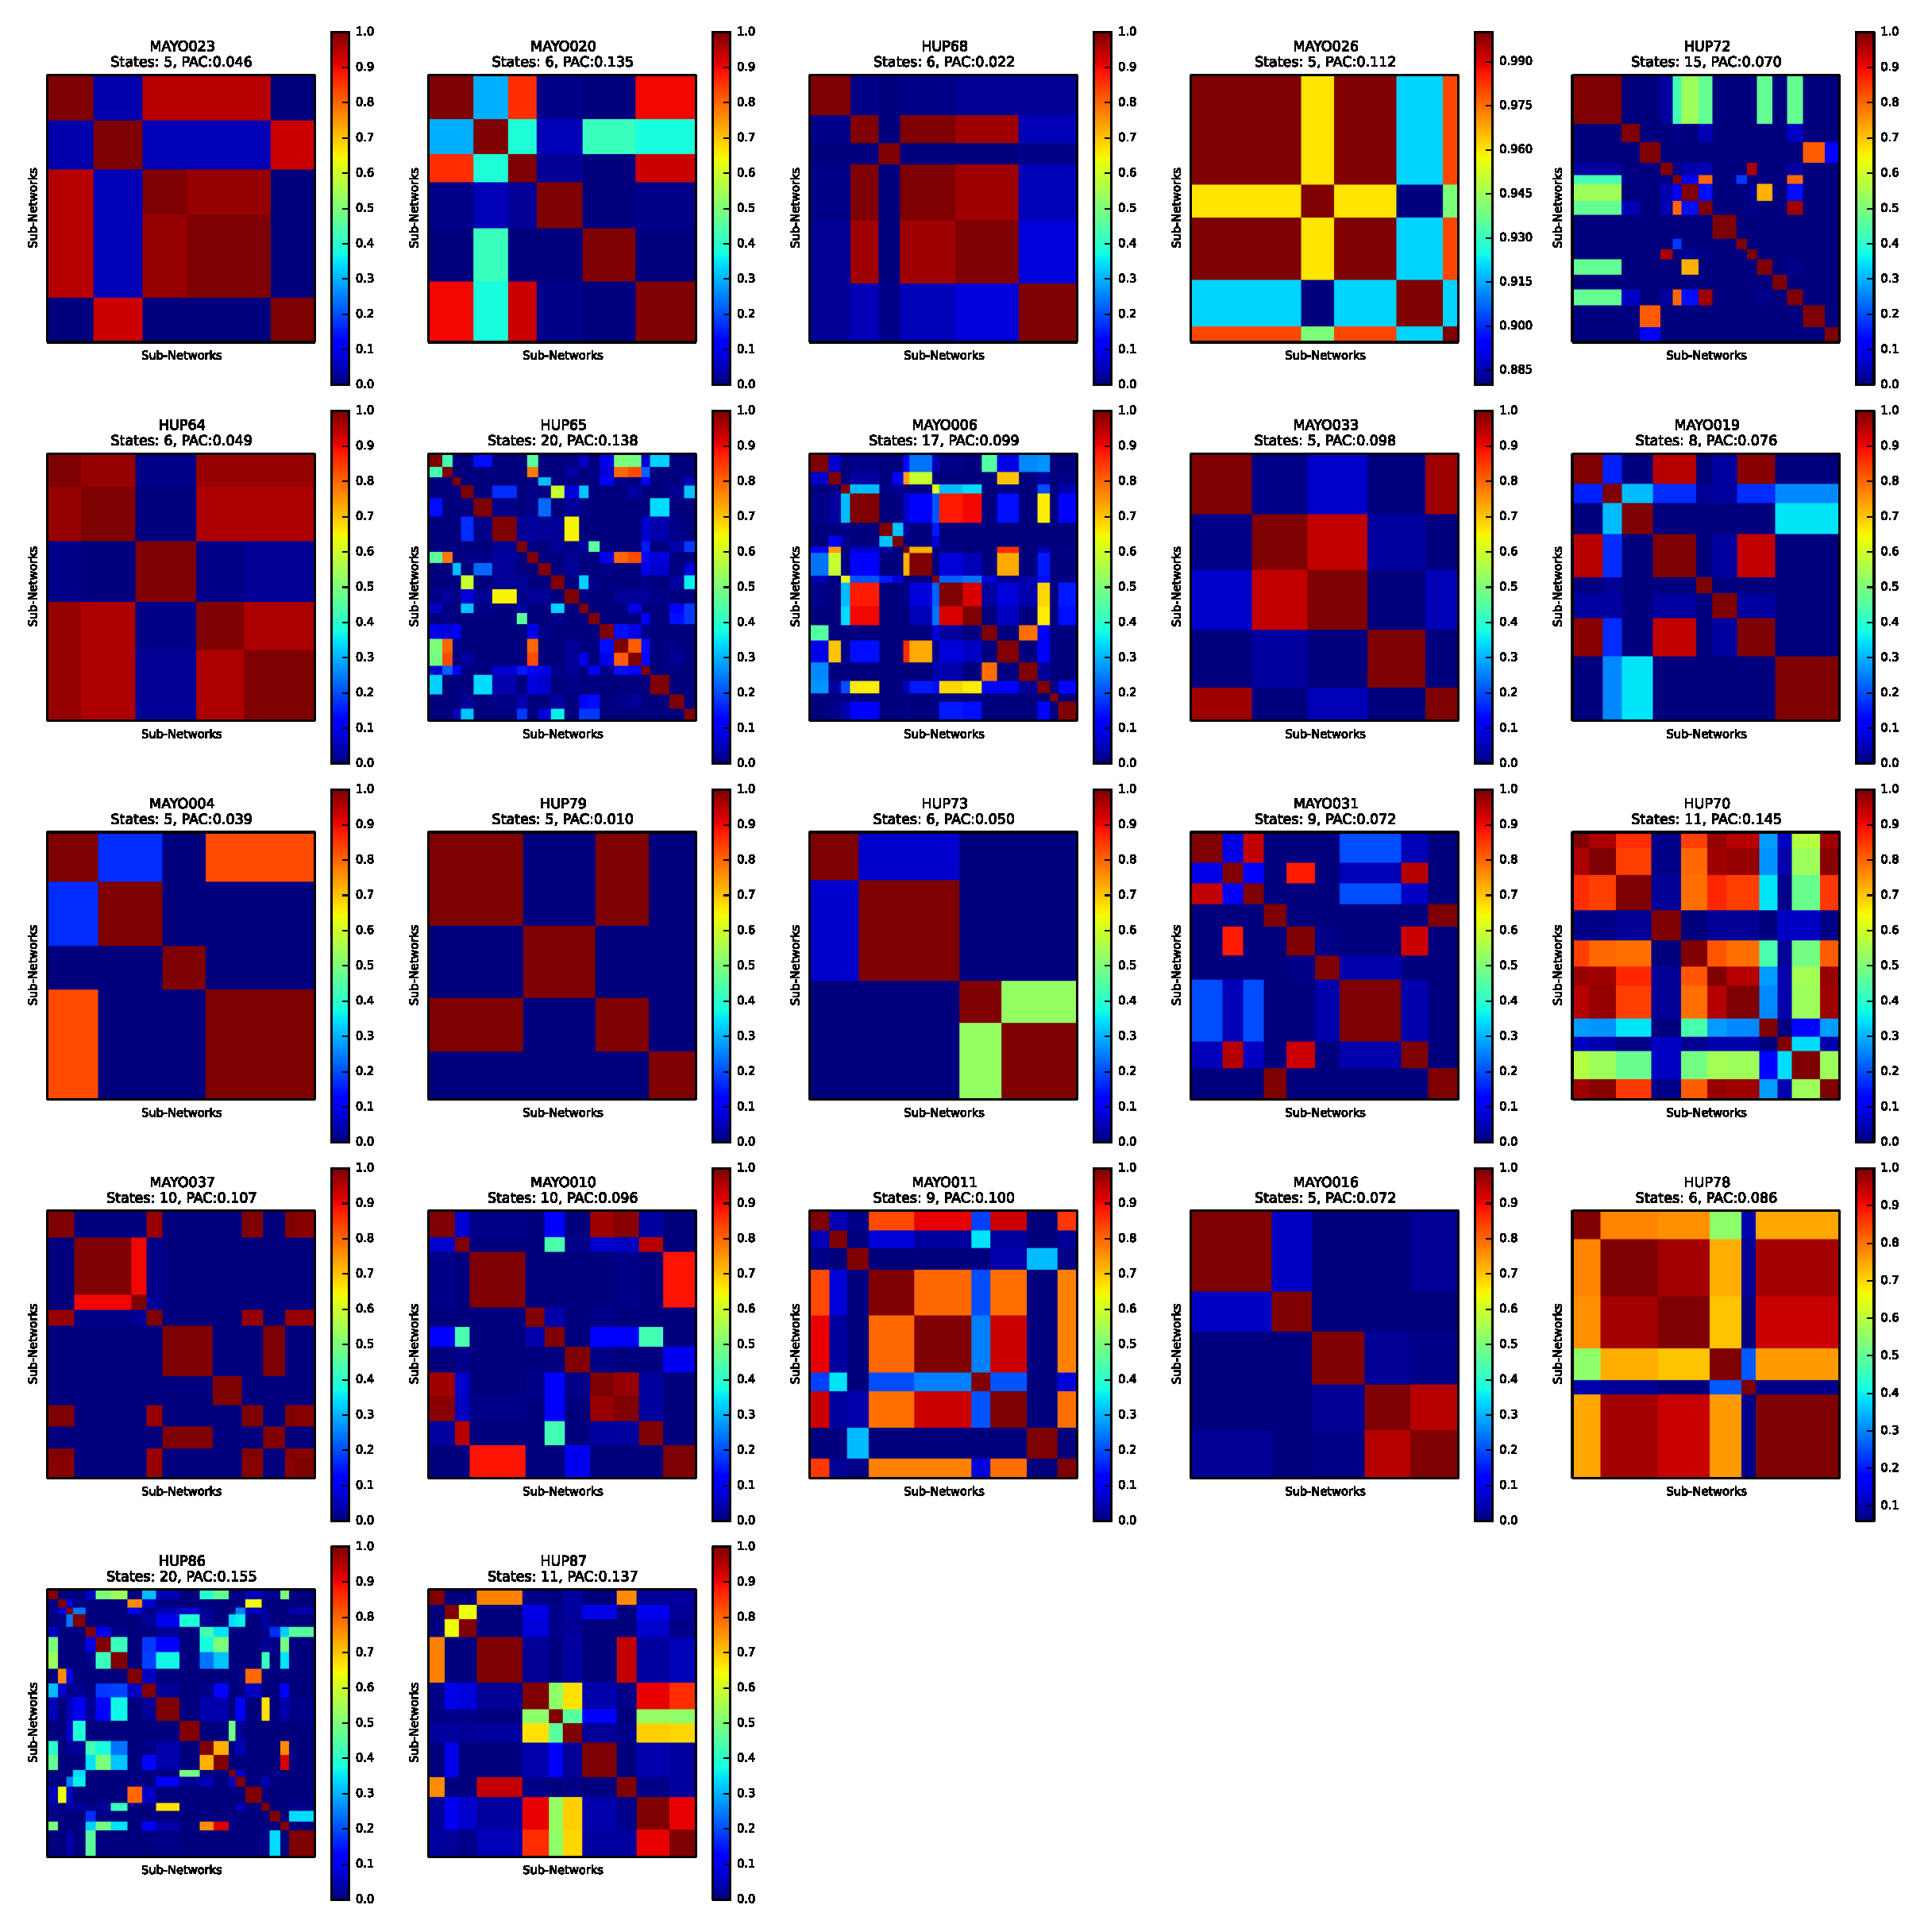
\includegraphics[width=\textwidth]{assign_true_cluster.eps}
    \caption[Co-clustering probability of ictal and interictal sub-networks]{\textbf{Optimum co-clustering probability of sub-networks.} For each patient, we assigned each ictal and interictal sub-network to a consensus cluster and re-ordered the co-clustering probability based on assigned clusters. We observed high co-clustering probability between clusters of sub-networks (block diagonal elements) and low co-clustering probability between clusters (off-diagonal blocks). \label{ch4:figS3}}
\end{figure}
